\section{Probability Distributions}

A random variable is function whose domain is the sample space of an
experiment, but random variables with that show up in completely different
experiments wind up behaving in much the same way because they have the
same probabilities of taking different values.  Namely, random variables
on different probability spaces may wind up having the same probability
density function.

\begin{definition}
Let $R$ be a random variable with with codomain $V$.
The \term{probability density function (pdf)} of $R$
is a function $\pdf_R : V \to [0,1]$ defined by:
%
\[
\pdf_R(x) \eqdef \begin{cases}
            \pr{R = x} & \text{if } x \in \range{R},\\
             0 & \text{if } x \notin \range{R}.
           \end{cases}
\]
\end{definition}
%
A consequence of this definition is that
%
\[
\sum_{x \in \range{R}} \pdf_R(x) = 1.
\]
This follows because $R$ has a value for each outcome, so summing the
probabilities over all outcomes is the same as summing over the
probabilities of each value in the range of $R$.

As an example, let's return to the experiment of rolling two fair,
independent dice.  As before, let $T$ be the total of the two rolls.
This random variable takes on values in the set $V = \set{2, 3,
\dots, 12}$.  A plot of the probability density function is shown
below:
%
\begin{center}
\begin{picture}(305,110)(-75,-40)
%\put(-75,-40){\dashbox(305,110)} % bounding box
\put(0,0){\vector(1,0){230}}
\put(0,0){\vector(0,1){70}}
\put(-1,60){\line(1,0){2}}
\put(-15,60){\makebox(0,0){{\small $6/36$}}}
\put(-1,30){\line(1,0){2}}
\put(-15,30){\makebox(0,0){{\small $3/36$}}}
\put(-50,40){\makebox(0,0){$\pdf_R(x)$}}
\put(120,-30){\makebox(0,0){$x \in V$}}
\put(0,0){\framebox(20,10){}}
\put(10,-10){\makebox(0,0){2}}
\put(20,0){\framebox(20,20){}}
\put(30,-10){\makebox(0,0){3}}
\put(40,0){\framebox(20,30){}}
\put(50,-10){\makebox(0,0){4}}
\put(60,0){\framebox(20,40){}}
\put(70,-10){\makebox(0,0){5}}
\put(80,0){\framebox(20,50){}}
\put(90,-10){\makebox(0,0){6}}
\put(100,0){\framebox(20,60){}}
\put(110,-10){\makebox(0,0){7}}
\put(120,0){\framebox(20,50){}}
\put(130,-10){\makebox(0,0){8}}
\put(140,0){\framebox(20,40){}}
\put(150,-10){\makebox(0,0){9}}
\put(160,0){\framebox(20,30){}}
\put(170,-10){\makebox(0,0){10}}
\put(180,0){\framebox(20,20){}}
\put(190,-10){\makebox(0,0){11}}
\put(200,0){\framebox(20,10){}}
\put(210,-10){\makebox(0,0){12}}
\end{picture}
\end{center}
%
The lump in the middle indicates that sums close to 7 are the most
likely.  The total area of all the rectangles is 1 since the dice must
take on exactly one of the sums in $V = \set{2, 3, \dots, 12}$.

A closely-related idea is the \term{cumulative distribution function
(cdf)} for a random variable $R$ whose codomain is real numbers.  This is a
function $\cdf_R : \reals \to [0,1]$ defined by:
%
\[
\cdf_R(x) = \pr{R \leq x}
\]
%
As an example, the cumulative distribution function for the random
variable $T$ is shown below:
%
\begin{center}
\begin{picture}(305,155)(-75,-40)
%\put(-75,-40){\dashbox(305,155)} % bounding box
\put(0,0){\vector(1,0){230}}
\put(0,0){\vector(0,1){115}}
\put(-1,108){\line(1,0){2}}
\put(-15,108){\makebox(0,0){{\small $1$}}}
\put(-1,54){\line(1,0){2}}
\put(-15,54){\makebox(0,0){{\small $1/2$}}}
\put(-15,0){\makebox(0,0){{\small $0$}}}
\put(-50,81){\makebox(0,0){$\cdf_R(x)$}}
\put(120,-30){\makebox(0,0){$x \in V$}}
\put(0,0){\framebox(20,3){}}
\put(10,-10){\makebox(0,0){2}}
\put(20,0){\framebox(20,9){}}
\put(30,-10){\makebox(0,0){3}}
\put(40,0){\framebox(20,18){}}
\put(50,-10){\makebox(0,0){4}}
\put(60,0){\framebox(20,30){}}
\put(70,-10){\makebox(0,0){5}}
\put(80,0){\framebox(20,45){}}
\put(90,-10){\makebox(0,0){6}}
\put(100,0){\framebox(20,63){}}
\put(110,-10){\makebox(0,0){7}}
\put(120,0){\framebox(20,78){}}
\put(130,-10){\makebox(0,0){8}}
\put(140,0){\framebox(20,90){}}
\put(150,-10){\makebox(0,0){9}}
\put(160,0){\framebox(20,99){}}
\put(170,-10){\makebox(0,0){10}}
\put(180,0){\framebox(20,105){}}
\put(190,-10){\makebox(0,0){11}}
\put(200,0){\framebox(20,108){}}
\put(210,-10){\makebox(0,0){12}}
\end{picture}
\end{center}
%
The height of the $i$-th bar in the cumulative distribution function
is equal to the \textit{sum} of the heights of the leftmost $i$ bars
in the probability density function.  This follows from the
definitions of pdf and cdf:
%
\begin{align*}
\cdf_R(x) & = \pr{R \leq x} \\
          & = \sum_{y \leq x} \pr{R = y} \\
          & = \sum_{y \leq x} \pdf_R(y)
\end{align*}

In summary, $\pdf_R(x)$ measures the probability that $R = x$ and
$\cdf_R(x)$ measures the probability that $R \leq x$.  Both the
$\pdf_R$ and $\cdf_R$ capture the same information about the random
variable $R$--- you can derive one from the other ---but sometimes one
is more convenient.  The key point here is that neither the
probability density function nor the cumulative distribution function
involves the sample space of an experiment.

\iffalse
Thus, through these
functions, we can study random variables without reference to a
particular experiment.
\fi


We'll now look at three important distributions and some applications.

\subsection{Bernoulli Distribution}

Indicator random variables are perhaps the most common type because of
their close association with events.  The probability density function
of an indicator random variable $B$ is always
%
\begin{align*}
\pdf_B(0) & = p \\
\pdf_B(1) & = 1 - p \\
\end{align*}
%
where $0 \leq p \leq 1$.  The corresponding cumulative distribution
function is:
%
\begin{align*}
\cdf_B(0) & = p \\
\cdf_B(1) & = 1
\end{align*}
%
%This is called the \term{Bernoulli distribution}. 
%The number of heads
%flipped on a (possibly biased) coin has a Bernoulli distribution.

\subsection{Uniform Distribution}

A random variable that takes on each possible value with the same
probability is called \term{uniform}.  For example, the probability
density function of a random variable $U$ that is uniform on the set
$\set{1, 2, \dots, N}$ is:
%
\begin{align*}
\pdf_U(k) = \frac{1}{N}
\end{align*}
%
And the cumulative distribution function is:
%
\begin{align*}
\cdf_U(k) = \frac{k}{N}
\end{align*}
%
Uniform distributions come up all the time.  For example, the number
rolled on a fair die is uniform on the set $\set{1, 2, \dots, 6}$.

\iffalse

\subsection{The Numbers Game}

Let's play a game!  I have two envelopes.  Each contains an integer in
the range $0, 1, \dots, 100$, and the numbers are distinct.  To win
the game, you must determine which envelope contains the larger
number.  To give you a fighting chance, I'll let you peek at the
number in one envelope selected at random.  Can you devise a strategy
that gives you a better than 50\% chance of winning?

For example, you could just pick an evelope at random and guess that
it contains the larger number.  But this strategy wins only 50\% of
the time.  Your challenge is to do better.

So you might try to be more clever.  Suppose you peek in the left
envelope and see the number 12.  Since 12 is a small number, you might
guess that that other number is larger.  But perhaps I'm sort of
tricky and put small numbers in \textit{both} envelopes.  Then your
guess might not be so good!

An important point here is that the numbers in the envelopes may
\textit{not} be random.  I'm picking the numbers and I'm choosing them
in a way that I think will defeat your guessing strategy.  I'll only
use randomization to choose the numbers if that serves \textit{my}
end:  making you lose!

\subsubsection{Intuition Behind the Winning Strategy}

Amazingly, there is a strategy that wins more than 50\% of the time,
regardless of what numbers I put in the envelopes!

Suppose that you somehow knew a number $x$ \textit{between} my lower
number and higher numbers.  Now you peek in an envelope and see one or
the other.  If it is bigger than $x$, then you know you're peeking at
the higher number.  If it is smaller than $x$, then you're peeking at
the lower number.  In other words, if you know a number $x$ between
my lower and higher numbers, then you are certain to win the game.

The only flaw with this brilliant strategy is that you do \textit{not}
know $x$.  Oh well.

But what if you try to \textit{guess} $x$?  There is some probability
that you guess correctly.  In this case, you win 100\% of the time.
On the other hand, if you guess incorrectly, then you're no worse off
than before; your chance of winning is still 50\%.  Combining these
two cases, your overall chance of winning is better than 50\%!

Informal arguments about probability, like this one, often sound
plausible, but do not hold up under close scrutiny.  In contrast, this
argument sounds completely implausible--- but is actually correct!

\subsubsection{Analysis of the Winning Strategy}

For generality, suppose that I can choose numbers from the set
$\set{0, 1, \dots, n}$.  Call the lower number $L$ and the higher
number $H$.

Your goal is to guess a number $x$ between $L$ and $H$.  To avoid
confusing equality cases, you select $x$ at random from among the
half-integers:
%
\[
\set{\frac{1}{2},\ 1\frac{1}{2},\ 2\frac{1}{2},\ \dots,\ n - \frac{1}{2}}
\]
%
But what probability distribution should you use?

The uniform distribution turns out to be your best bet.  An informal
justification is that if I figured out that you were unlikely to pick
some number--- say $50\frac{1}{2}$--- then I'd always put 50 and 51 in
the evelopes.  Then you'd be unlikely to pick an $x$ between $L$ and
$H$ and would have less chance of winning.

After you've selected the number $x$, you peek into an envelope and
see some number $p$.  If $p > x$, then you guess that you're looking
at the larger number.  If $p < x$, then you guess that the other
number is larger.

All that remains is to determine the probability that this strategy
succeeds.  We can do this with the usual four step method and a tree
diagram.

\noindent \textbf{Step 1: Find the sample space. }  You either choose
$x$ too low ($< L$), too high ($> H$), or just right ($L < x < H$).
Then you either peek at the lower number ($p = L$) or the higher
number ($p = H$).  This gives a total of six possible outcomes.
%
\begin{center}
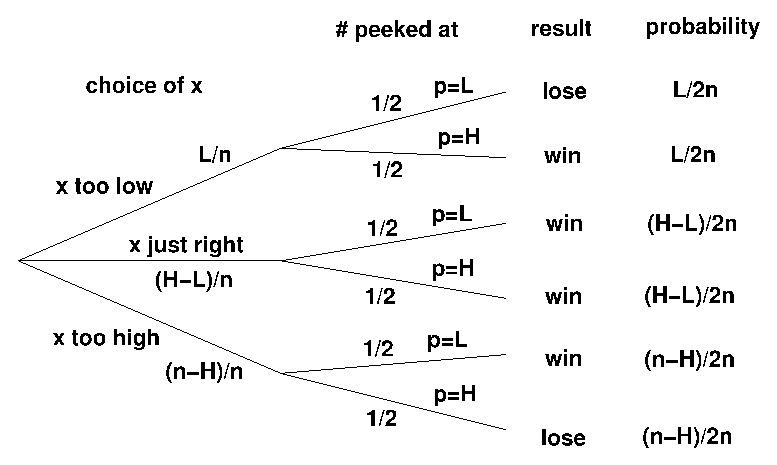
\includegraphics[height=2.5in]{figures/numbers-game}
\end{center}

\noindent \textbf{Step 2: Define events of interest. } The four
outcomes in the event that you win are marked in the tree diagram.

\noindent \textbf{Step 3: Assign outcome probabilities. } First, we
assign edge probabilities.  Your guess $x$ is too low with probability
$L/n$, too high with probability $(n-H)/n$, and just right with
probability $(H-L)/n$.  Next, you peek at either the lower or higher
number with equal probability.  Multiplying along root-to-leaf paths
gives the outcome probabilities.

\noindent \textbf{Step 4: Compute event probabilities. }  The
probability of the event that you win is the sum of the probabilities
of the four outcomes in that event:
%
\begin{align*}
\pr{\text{win}}
    & = \frac{L}{2n} + \frac{H-L}{2n} + \frac{H-L}{2n}  + \frac{n-H}{2n} \\
    & = \frac{1}{2} + \frac{H-L}{2n} \\
    & \geq \frac{1}{2} + \frac{1}{2n}
\end{align*}
%
The final inequality relies on the fact that the higher number $H$ is
at least 1 greater than the lower number $L$ since they are required
to be distinct.

Sure enough, you win with this strategy more than half the time,
regardless of the numbers in the envelopes!  For example, if I choose
numbers in the range $0, 1, \dots, 100$, then you win with probability at
least $\frac{1}{2} + \frac{1}{200} = 50.5\%$.  Even better, if I'm allowed
only numbers in the range $0, \dots, 10$, then your probability of
winning rises to 55\%!  By Las Vegas standards, those are great odds!
\fi

\subsection{Binomial Distribution}

Of the more complex distributions, the \term{binomial distribution} is
surely the most important in Computer Science.  The standard example
of a random variable with a binomial distribution is the number of
heads that come up in $n$ independent flips of a coin; call this
random variable $H_n$.  If the coin is fair, then $H_n$ has an
\textit{unbiased binomial density function}:
%
\[
\pdf_{H_n}(k) = \binom{n}{k} 2^{-n}.
\]
%
This follows because there are $\binom{n}{k}$ sequences of $n$ coin
tosses with exactly $k$ heads, and each such sequence has probability
$2^{-n}$.

Here is a plot of the unbiased probability density function
$\pdf_{H_n}(k)$ corresponding to $n = 20$ coins flips.  The most likely
outcome is $k = 10$ heads, and the probability falls off rapidly for
larger and smaller values of $k$.  These falloff regions to the left and
right of the main hump are usually called the \term{tails of the
distribution}.
%
\begin{center}
% GNUPLOT: LaTeX picture
\setlength{\unitlength}{0.240900pt}
\ifx\plotpoint\undefined\newsavebox{\plotpoint}\fi
\sbox{\plotpoint}{\rule[-0.200pt]{0.400pt}{0.400pt}}%
\begin{picture}(1500,900)(0,0)
\font\gnuplot=cmr10 at 10pt
\gnuplot
\sbox{\plotpoint}{\rule[-0.200pt]{0.400pt}{0.400pt}}%
\put(140.0,82.0){\rule[-0.200pt]{4.818pt}{0.400pt}}
\put(120,82){\makebox(0,0)[r]{0}}
\put(1419.0,82.0){\rule[-0.200pt]{4.818pt}{0.400pt}}
\put(140.0,168.0){\rule[-0.200pt]{4.818pt}{0.400pt}}
\put(120,168){\makebox(0,0)[r]{0.02}}
\put(1419.0,168.0){\rule[-0.200pt]{4.818pt}{0.400pt}}
\put(140.0,255.0){\rule[-0.200pt]{4.818pt}{0.400pt}}
\put(120,255){\makebox(0,0)[r]{0.04}}
\put(1419.0,255.0){\rule[-0.200pt]{4.818pt}{0.400pt}}
\put(140.0,341.0){\rule[-0.200pt]{4.818pt}{0.400pt}}
\put(120,341){\makebox(0,0)[r]{0.06}}
\put(1419.0,341.0){\rule[-0.200pt]{4.818pt}{0.400pt}}
\put(140.0,428.0){\rule[-0.200pt]{4.818pt}{0.400pt}}
\put(120,428){\makebox(0,0)[r]{0.08}}
\put(1419.0,428.0){\rule[-0.200pt]{4.818pt}{0.400pt}}
\put(140.0,514.0){\rule[-0.200pt]{4.818pt}{0.400pt}}
\put(120,514){\makebox(0,0)[r]{0.1}}
\put(1419.0,514.0){\rule[-0.200pt]{4.818pt}{0.400pt}}
\put(140.0,601.0){\rule[-0.200pt]{4.818pt}{0.400pt}}
\put(120,601){\makebox(0,0)[r]{0.12}}
\put(1419.0,601.0){\rule[-0.200pt]{4.818pt}{0.400pt}}
\put(140.0,687.0){\rule[-0.200pt]{4.818pt}{0.400pt}}
\put(120,687){\makebox(0,0)[r]{0.14}}
\put(1419.0,687.0){\rule[-0.200pt]{4.818pt}{0.400pt}}
\put(140.0,774.0){\rule[-0.200pt]{4.818pt}{0.400pt}}
\put(120,774){\makebox(0,0)[r]{0.16}}
\put(1419.0,774.0){\rule[-0.200pt]{4.818pt}{0.400pt}}
\put(140.0,860.0){\rule[-0.200pt]{4.818pt}{0.400pt}}
\put(120,860){\makebox(0,0)[r]{0.18}}
\put(1419.0,860.0){\rule[-0.200pt]{4.818pt}{0.400pt}}
\put(140.0,82.0){\rule[-0.200pt]{0.400pt}{4.818pt}}
\put(140,41){\makebox(0,0){0}}
\put(140.0,840.0){\rule[-0.200pt]{0.400pt}{4.818pt}}
\put(465.0,82.0){\rule[-0.200pt]{0.400pt}{4.818pt}}
\put(465,41){\makebox(0,0){5}}
\put(465.0,840.0){\rule[-0.200pt]{0.400pt}{4.818pt}}
\put(790.0,82.0){\rule[-0.200pt]{0.400pt}{4.818pt}}
\put(790,41){\makebox(0,0){10}}
\put(790.0,840.0){\rule[-0.200pt]{0.400pt}{4.818pt}}
\put(1114.0,82.0){\rule[-0.200pt]{0.400pt}{4.818pt}}
\put(1114,41){\makebox(0,0){15}}
\put(1114.0,840.0){\rule[-0.200pt]{0.400pt}{4.818pt}}
\put(1439.0,82.0){\rule[-0.200pt]{0.400pt}{4.818pt}}
\put(1439,41){\makebox(0,0){20}}
\put(1439.0,840.0){\rule[-0.200pt]{0.400pt}{4.818pt}}
\put(140.0,82.0){\rule[-0.200pt]{312.929pt}{0.400pt}}
\put(1439.0,82.0){\rule[-0.200pt]{0.400pt}{187.420pt}}
\put(140.0,860.0){\rule[-0.200pt]{312.929pt}{0.400pt}}
\put(140.0,82.0){\rule[-0.200pt]{0.400pt}{187.420pt}}
\put(140,82){\usebox{\plotpoint}}
\put(140.0,82.0){\rule[-0.200pt]{25.294pt}{0.400pt}}
\put(245.0,82.0){\usebox{\plotpoint}}
\put(245.0,83.0){\rule[-0.200pt]{15.899pt}{0.400pt}}
\put(311.0,83.0){\rule[-0.200pt]{0.400pt}{0.964pt}}
\put(311.0,87.0){\rule[-0.200pt]{15.658pt}{0.400pt}}
\put(376.0,87.0){\rule[-0.200pt]{0.400pt}{3.613pt}}
\put(376.0,102.0){\rule[-0.200pt]{15.899pt}{0.400pt}}
\put(442.0,102.0){\rule[-0.200pt]{0.400pt}{10.600pt}}
\put(442.0,146.0){\rule[-0.200pt]{15.658pt}{0.400pt}}
\put(507.0,146.0){\rule[-0.200pt]{0.400pt}{23.126pt}}
\put(507.0,242.0){\rule[-0.200pt]{15.899pt}{0.400pt}}
\put(573.0,242.0){\rule[-0.200pt]{0.400pt}{38.544pt}}
\put(573.0,402.0){\rule[-0.200pt]{15.899pt}{0.400pt}}
\put(639.0,402.0){\rule[-0.200pt]{0.400pt}{47.939pt}}
\put(639.0,601.0){\rule[-0.200pt]{15.658pt}{0.400pt}}
\put(704.0,601.0){\rule[-0.200pt]{0.400pt}{41.676pt}}
\put(704.0,774.0){\rule[-0.200pt]{15.899pt}{0.400pt}}
\put(770.0,774.0){\rule[-0.200pt]{0.400pt}{16.863pt}}
\put(770.0,844.0){\rule[-0.200pt]{12.527pt}{0.400pt}}
\put(822.0,774.0){\rule[-0.200pt]{0.400pt}{16.863pt}}
\put(822.0,774.0){\rule[-0.200pt]{15.899pt}{0.400pt}}
\put(888.0,601.0){\rule[-0.200pt]{0.400pt}{41.676pt}}
\put(888.0,601.0){\rule[-0.200pt]{15.899pt}{0.400pt}}
\put(954.0,402.0){\rule[-0.200pt]{0.400pt}{47.939pt}}
\put(954.0,402.0){\rule[-0.200pt]{15.658pt}{0.400pt}}
\put(1019.0,242.0){\rule[-0.200pt]{0.400pt}{38.544pt}}
\put(1019.0,242.0){\rule[-0.200pt]{15.899pt}{0.400pt}}
\put(1085.0,146.0){\rule[-0.200pt]{0.400pt}{23.126pt}}
\put(1085.0,146.0){\rule[-0.200pt]{15.658pt}{0.400pt}}
\put(1150.0,102.0){\rule[-0.200pt]{0.400pt}{10.600pt}}
\put(1150.0,102.0){\rule[-0.200pt]{15.899pt}{0.400pt}}
\put(1216.0,87.0){\rule[-0.200pt]{0.400pt}{3.613pt}}
\put(1216.0,87.0){\rule[-0.200pt]{15.899pt}{0.400pt}}
\put(1282.0,83.0){\rule[-0.200pt]{0.400pt}{0.964pt}}
\put(1282.0,83.0){\rule[-0.200pt]{15.658pt}{0.400pt}}
\put(1347.0,82.0){\usebox{\plotpoint}}
\put(1347.0,82.0){\rule[-0.200pt]{22.163pt}{0.400pt}}
\end{picture}
\end{center}
%
An enormous number of analyses in Computer Science come down to proving
that the tails of the binomial and similar distributions are very small.
In the context of a problem, this typically means that there is very small
probability that something \textit{bad} happens, which could be a server
or communication link overloading or a randomized algorithm running for an
exceptionally long time or producing the wrong result.

\subsubsection{The General Binomial Distribution}

Now let $J$ be the number of heads that come up on $n$ independent
coins, each of which is heads with probability $p$.  Then $J$ has a
\textit{general binomial density function}:
%
\[
\pdf_J(k) = \binom{n}{k} p^k (1-p)^{n-k}.
\]
%
As before, there are $\binom{n}{k}$ sequences with $k$ heads and $n -
k$ tails, but now the probability of each such sequence is $p^k
(1-p)^{n-k}$.

As an example, the plot below shows the probability density function
$\pdf_J(k)$ corresponding to flipping $n=20$ independent coins that
are heads with probabilty $p = 0.75$.  The graph shows that we are
most likely to get around $k = 15$ heads, as you might expect.  Once
again, the probability falls off quickly for larger and smaller values
of $k$.
%
\begin{center}
% GNUPLOT: LaTeX picture
\setlength{\unitlength}{0.240900pt}
\ifx\plotpoint\undefined\newsavebox{\plotpoint}\fi
\sbox{\plotpoint}{\rule[-0.200pt]{0.400pt}{0.400pt}}%
\begin{picture}(1500,900)(0,0)
\font\gnuplot=cmr10 at 10pt
\gnuplot
\sbox{\plotpoint}{\rule[-0.200pt]{0.400pt}{0.400pt}}%
\put(140.0,82.0){\rule[-0.200pt]{4.818pt}{0.400pt}}
\put(120,82){\makebox(0,0)[r]{0}}
\put(1419.0,82.0){\rule[-0.200pt]{4.818pt}{0.400pt}}
\put(140.0,238.0){\rule[-0.200pt]{4.818pt}{0.400pt}}
\put(120,238){\makebox(0,0)[r]{0.05}}
\put(1419.0,238.0){\rule[-0.200pt]{4.818pt}{0.400pt}}
\put(140.0,393.0){\rule[-0.200pt]{4.818pt}{0.400pt}}
\put(120,393){\makebox(0,0)[r]{0.1}}
\put(1419.0,393.0){\rule[-0.200pt]{4.818pt}{0.400pt}}
\put(140.0,549.0){\rule[-0.200pt]{4.818pt}{0.400pt}}
\put(120,549){\makebox(0,0)[r]{0.15}}
\put(1419.0,549.0){\rule[-0.200pt]{4.818pt}{0.400pt}}
\put(140.0,704.0){\rule[-0.200pt]{4.818pt}{0.400pt}}
\put(120,704){\makebox(0,0)[r]{0.2}}
\put(1419.0,704.0){\rule[-0.200pt]{4.818pt}{0.400pt}}
\put(140.0,860.0){\rule[-0.200pt]{4.818pt}{0.400pt}}
\put(120,860){\makebox(0,0)[r]{0.25}}
\put(1419.0,860.0){\rule[-0.200pt]{4.818pt}{0.400pt}}
\put(140.0,82.0){\rule[-0.200pt]{0.400pt}{4.818pt}}
\put(140,41){\makebox(0,0){0}}
\put(140.0,840.0){\rule[-0.200pt]{0.400pt}{4.818pt}}
\put(449.0,82.0){\rule[-0.200pt]{0.400pt}{4.818pt}}
\put(449,41){\makebox(0,0){5}}
\put(449.0,840.0){\rule[-0.200pt]{0.400pt}{4.818pt}}
\put(759.0,82.0){\rule[-0.200pt]{0.400pt}{4.818pt}}
\put(759,41){\makebox(0,0){10}}
\put(759.0,840.0){\rule[-0.200pt]{0.400pt}{4.818pt}}
\put(1068.0,82.0){\rule[-0.200pt]{0.400pt}{4.818pt}}
\put(1068,41){\makebox(0,0){15}}
\put(1068.0,840.0){\rule[-0.200pt]{0.400pt}{4.818pt}}
\put(1377.0,82.0){\rule[-0.200pt]{0.400pt}{4.818pt}}
\put(1377,41){\makebox(0,0){20}}
\put(1377.0,840.0){\rule[-0.200pt]{0.400pt}{4.818pt}}
\put(140.0,82.0){\rule[-0.200pt]{312.929pt}{0.400pt}}
\put(1439.0,82.0){\rule[-0.200pt]{0.400pt}{187.420pt}}
\put(140.0,860.0){\rule[-0.200pt]{312.929pt}{0.400pt}}
\put(140.0,82.0){\rule[-0.200pt]{0.400pt}{187.420pt}}
\put(140,82){\usebox{\plotpoint}}
\put(140.0,82.0){\rule[-0.200pt]{113.705pt}{0.400pt}}
\put(612.0,82.0){\rule[-0.200pt]{0.400pt}{0.482pt}}
\put(612.0,84.0){\rule[-0.200pt]{15.899pt}{0.400pt}}
\put(678.0,84.0){\rule[-0.200pt]{0.400pt}{1.686pt}}
\put(678.0,91.0){\rule[-0.200pt]{12.527pt}{0.400pt}}
\put(730.0,91.0){\rule[-0.200pt]{0.400pt}{5.300pt}}
\put(730.0,113.0){\rule[-0.200pt]{15.899pt}{0.400pt}}
\put(796.0,113.0){\rule[-0.200pt]{0.400pt}{12.768pt}}
\put(796.0,166.0){\rule[-0.200pt]{15.899pt}{0.400pt}}
\put(862.0,166.0){\rule[-0.200pt]{0.400pt}{25.294pt}}
\put(862.0,271.0){\rule[-0.200pt]{12.527pt}{0.400pt}}
\put(914.0,271.0){\rule[-0.200pt]{0.400pt}{38.785pt}}
\put(914.0,432.0){\rule[-0.200pt]{15.899pt}{0.400pt}}
\put(980.0,432.0){\rule[-0.200pt]{0.400pt}{42.157pt}}
\put(980.0,607.0){\rule[-0.200pt]{15.658pt}{0.400pt}}
\put(1045.0,607.0){\rule[-0.200pt]{0.400pt}{25.294pt}}
\put(1045.0,712.0){\rule[-0.200pt]{15.899pt}{0.400pt}}
\put(1111.0,672.0){\rule[-0.200pt]{0.400pt}{9.636pt}}
\put(1111.0,672.0){\rule[-0.200pt]{12.527pt}{0.400pt}}
\put(1163.0,499.0){\rule[-0.200pt]{0.400pt}{41.676pt}}
\put(1163.0,499.0){\rule[-0.200pt]{15.899pt}{0.400pt}}
\put(1229.0,290.0){\rule[-0.200pt]{0.400pt}{50.348pt}}
\put(1229.0,290.0){\rule[-0.200pt]{15.899pt}{0.400pt}}
\put(1295.0,148.0){\rule[-0.200pt]{0.400pt}{34.208pt}}
\put(1295.0,148.0){\rule[-0.200pt]{12.527pt}{0.400pt}}
\put(1347.0,92.0){\rule[-0.200pt]{0.400pt}{13.490pt}}
\put(1347.0,92.0){\rule[-0.200pt]{15.899pt}{0.400pt}}
\put(1413.0,83.0){\rule[-0.200pt]{0.400pt}{2.168pt}}
\put(1413.0,83.0){\rule[-0.200pt]{6.263pt}{0.400pt}}
\end{picture}
\end{center}

\subsubsection{Approximating the Binomial Density Function}

Computing the general binomial density function is daunting if not
impossible when $n$ is up in the thousands.  Fortunately, there is an
approximate closed-form formula for this function based on
an approximation for the binomial coefficient.  In the formula, $k$ is
replaced by $\alpha n$ where $\alpha$ is a number between 0 and 1.
%
\begin{lemma}\label{LN12:bincoeff-bound}
\begin{align*}
\binom{n}{\alpha n}
        & \leq \frac{2^{n H(\alpha)}}{\sqrt{2 \pi \alpha (1 - \alpha) n}}
\end{align*}
%
where $H(\alpha)$ is the famous \term{entropy function}:
%
\[
H(\alpha) \eqdef \alpha \log_2 \frac{1}{\alpha} +
                (1 - \alpha) \log_2 \frac{1}{1 - \alpha}
\]
\end{lemma}

%
The graph of $H$ is shown in Figure~\ref{LN12:entropy}.

                                % GNUPLOT: LaTeX picture
\begin{figure}
\setlength{\unitlength}{0.240900pt}
\ifx\plotpoint\undefined\newsavebox{\plotpoint}\fi
\sbox{\plotpoint}{\rule[-0.200pt]{0.400pt}{0.400pt}}%
\begin{picture}(1500,900)(0,0)
  \font\gnuplot=cmr10 at 10pt
  \gnuplot
  \sbox{\plotpoint}{\rule[-0.200pt]{0.400pt}{0.400pt}}%
  \put(220.0,113.0){\rule[-0.200pt]{292.934pt}{0.400pt}}
  \put(220.0,113.0){\rule[-0.200pt]{0.400pt}{184.048pt}}
  \put(220.0,113.0){\rule[-0.200pt]{4.818pt}{0.400pt}}
  \put(198,113){\makebox(0,0)[r]{0}}
  \put(1416.0,113.0){\rule[-0.200pt]{4.818pt}{0.400pt}}
  \put(220.0,266.0){\rule[-0.200pt]{4.818pt}{0.400pt}}
  \put(198,266){\makebox(0,0)[r]{0.2}}
  \put(1416.0,266.0){\rule[-0.200pt]{4.818pt}{0.400pt}}
  \put(220.0,419.0){\rule[-0.200pt]{4.818pt}{0.400pt}}
  \put(198,419){\makebox(0,0)[r]{0.4}}
  \put(1416.0,419.0){\rule[-0.200pt]{4.818pt}{0.400pt}}
  \put(220.0,571.0){\rule[-0.200pt]{4.818pt}{0.400pt}}
  \put(198,571){\makebox(0,0)[r]{0.6}}
  \put(1416.0,571.0){\rule[-0.200pt]{4.818pt}{0.400pt}}
  \put(220.0,724.0){\rule[-0.200pt]{4.818pt}{0.400pt}}
  \put(198,724){\makebox(0,0)[r]{0.8}}
  \put(1416.0,724.0){\rule[-0.200pt]{4.818pt}{0.400pt}}
  \put(220.0,877.0){\rule[-0.200pt]{4.818pt}{0.400pt}}
  \put(198,877){\makebox(0,0)[r]{1}}
  \put(1416.0,877.0){\rule[-0.200pt]{4.818pt}{0.400pt}}
  \put(220.0,113.0){\rule[-0.200pt]{0.400pt}{4.818pt}}
  \put(220,68){\makebox(0,0){0}}
  \put(220.0,857.0){\rule[-0.200pt]{0.400pt}{4.818pt}}
  \put(463.0,113.0){\rule[-0.200pt]{0.400pt}{4.818pt}}
  \put(463,68){\makebox(0,0){0.2}}
  \put(463.0,857.0){\rule[-0.200pt]{0.400pt}{4.818pt}}
  \put(706.0,113.0){\rule[-0.200pt]{0.400pt}{4.818pt}}
  \put(706,68){\makebox(0,0){0.4}}
  \put(706.0,857.0){\rule[-0.200pt]{0.400pt}{4.818pt}}
  \put(950.0,113.0){\rule[-0.200pt]{0.400pt}{4.818pt}}
  \put(950,68){\makebox(0,0){0.6}}
  \put(950.0,857.0){\rule[-0.200pt]{0.400pt}{4.818pt}}
  \put(1193.0,113.0){\rule[-0.200pt]{0.400pt}{4.818pt}}
  \put(1193,68){\makebox(0,0){0.8}}
  \put(1193.0,857.0){\rule[-0.200pt]{0.400pt}{4.818pt}}
  \put(1436.0,113.0){\rule[-0.200pt]{0.400pt}{4.818pt}}
  \put(1436,68){\makebox(0,0){1}}
  \put(1436.0,857.0){\rule[-0.200pt]{0.400pt}{4.818pt}}
  \put(220.0,113.0){\rule[-0.200pt]{292.934pt}{0.400pt}}
  \put(1436.0,113.0){\rule[-0.200pt]{0.400pt}{184.048pt}}
  \put(220.0,877.0){\rule[-0.200pt]{292.934pt}{0.400pt}}
  \put(45,495){\makebox(0,0){$H(\alpha)$}}
  \put(828,23){\makebox(0,0){$\alpha$}}
  \put(220.0,113.0){\rule[-0.200pt]{0.400pt}{184.048pt}}
  \put(232,175){\usebox{\plotpoint}}
  \multiput(232.58,175.00)(0.493,1.845){23}{\rule{0.119pt}{1.546pt}}
  \multiput(231.17,175.00)(13.000,43.791){2}{\rule{0.400pt}{0.773pt}}
  \multiput(245.58,222.00)(0.492,1.746){21}{\rule{0.119pt}{1.467pt}}
  \multiput(244.17,222.00)(12.000,37.956){2}{\rule{0.400pt}{0.733pt}}
  \multiput(257.58,263.00)(0.492,1.573){21}{\rule{0.119pt}{1.333pt}}
  \multiput(256.17,263.00)(12.000,34.233){2}{\rule{0.400pt}{0.667pt}}
  \multiput(269.58,300.00)(0.492,1.401){21}{\rule{0.119pt}{1.200pt}}
  \multiput(268.17,300.00)(12.000,30.509){2}{\rule{0.400pt}{0.600pt}}
  \multiput(281.58,333.00)(0.493,1.250){23}{\rule{0.119pt}{1.085pt}}
  \multiput(280.17,333.00)(13.000,29.749){2}{\rule{0.400pt}{0.542pt}}
  \multiput(294.58,365.00)(0.492,1.272){21}{\rule{0.119pt}{1.100pt}}
  \multiput(293.17,365.00)(12.000,27.717){2}{\rule{0.400pt}{0.550pt}}
  \multiput(306.58,395.00)(0.492,1.142){21}{\rule{0.119pt}{1.000pt}}
  \multiput(305.17,395.00)(12.000,24.924){2}{\rule{0.400pt}{0.500pt}}
  \multiput(318.58,422.00)(0.493,1.052){23}{\rule{0.119pt}{0.931pt}}
  \multiput(317.17,422.00)(13.000,25.068){2}{\rule{0.400pt}{0.465pt}}
  \multiput(331.58,449.00)(0.492,1.056){21}{\rule{0.119pt}{0.933pt}}
  \multiput(330.17,449.00)(12.000,23.063){2}{\rule{0.400pt}{0.467pt}}
  \multiput(343.58,474.00)(0.492,0.970){21}{\rule{0.119pt}{0.867pt}}
  \multiput(342.17,474.00)(12.000,21.201){2}{\rule{0.400pt}{0.433pt}}
  \multiput(355.58,497.00)(0.492,0.970){21}{\rule{0.119pt}{0.867pt}}
  \multiput(354.17,497.00)(12.000,21.201){2}{\rule{0.400pt}{0.433pt}}
  \multiput(367.58,520.00)(0.493,0.853){23}{\rule{0.119pt}{0.777pt}}
  \multiput(366.17,520.00)(13.000,20.387){2}{\rule{0.400pt}{0.388pt}}
  \multiput(380.58,542.00)(0.492,0.841){21}{\rule{0.119pt}{0.767pt}}
  \multiput(379.17,542.00)(12.000,18.409){2}{\rule{0.400pt}{0.383pt}}
  \multiput(392.58,562.00)(0.492,0.841){21}{\rule{0.119pt}{0.767pt}}
  \multiput(391.17,562.00)(12.000,18.409){2}{\rule{0.400pt}{0.383pt}}
  \multiput(404.58,582.00)(0.493,0.734){23}{\rule{0.119pt}{0.685pt}}
  \multiput(403.17,582.00)(13.000,17.579){2}{\rule{0.400pt}{0.342pt}}
  \multiput(417.58,601.00)(0.492,0.712){21}{\rule{0.119pt}{0.667pt}}
  \multiput(416.17,601.00)(12.000,15.616){2}{\rule{0.400pt}{0.333pt}}
  \multiput(429.58,618.00)(0.492,0.755){21}{\rule{0.119pt}{0.700pt}}
  \multiput(428.17,618.00)(12.000,16.547){2}{\rule{0.400pt}{0.350pt}}
  \multiput(441.58,636.00)(0.492,0.669){21}{\rule{0.119pt}{0.633pt}}
  \multiput(440.17,636.00)(12.000,14.685){2}{\rule{0.400pt}{0.317pt}}
  \multiput(453.58,652.00)(0.493,0.616){23}{\rule{0.119pt}{0.592pt}}
  \multiput(452.17,652.00)(13.000,14.771){2}{\rule{0.400pt}{0.296pt}}
  \multiput(466.58,668.00)(0.492,0.625){21}{\rule{0.119pt}{0.600pt}}
  \multiput(465.17,668.00)(12.000,13.755){2}{\rule{0.400pt}{0.300pt}}
  \multiput(478.58,683.00)(0.492,0.582){21}{\rule{0.119pt}{0.567pt}}
  \multiput(477.17,683.00)(12.000,12.824){2}{\rule{0.400pt}{0.283pt}}
  \multiput(490.00,697.58)(0.497,0.493){23}{\rule{0.500pt}{0.119pt}}
  \multiput(490.00,696.17)(11.962,13.000){2}{\rule{0.250pt}{0.400pt}}
  \multiput(503.58,710.00)(0.492,0.539){21}{\rule{0.119pt}{0.533pt}}
  \multiput(502.17,710.00)(12.000,11.893){2}{\rule{0.400pt}{0.267pt}}
  \multiput(515.58,723.00)(0.492,0.539){21}{\rule{0.119pt}{0.533pt}}
  \multiput(514.17,723.00)(12.000,11.893){2}{\rule{0.400pt}{0.267pt}}
  \multiput(527.00,736.58)(0.496,0.492){21}{\rule{0.500pt}{0.119pt}}
  \multiput(527.00,735.17)(10.962,12.000){2}{\rule{0.250pt}{0.400pt}}
  \multiput(539.00,748.58)(0.590,0.492){19}{\rule{0.573pt}{0.118pt}}
  \multiput(539.00,747.17)(11.811,11.000){2}{\rule{0.286pt}{0.400pt}}
  \multiput(552.00,759.58)(0.600,0.491){17}{\rule{0.580pt}{0.118pt}}
  \multiput(552.00,758.17)(10.796,10.000){2}{\rule{0.290pt}{0.400pt}}
  \multiput(564.00,769.58)(0.543,0.492){19}{\rule{0.536pt}{0.118pt}}
  \multiput(564.00,768.17)(10.887,11.000){2}{\rule{0.268pt}{0.400pt}}
  \multiput(576.00,780.59)(0.669,0.489){15}{\rule{0.633pt}{0.118pt}}
  \multiput(576.00,779.17)(10.685,9.000){2}{\rule{0.317pt}{0.400pt}}
  \multiput(588.00,789.59)(0.728,0.489){15}{\rule{0.678pt}{0.118pt}}
  \multiput(588.00,788.17)(11.593,9.000){2}{\rule{0.339pt}{0.400pt}}
  \multiput(601.00,798.59)(0.669,0.489){15}{\rule{0.633pt}{0.118pt}}
  \multiput(601.00,797.17)(10.685,9.000){2}{\rule{0.317pt}{0.400pt}}
  \multiput(613.00,807.59)(0.758,0.488){13}{\rule{0.700pt}{0.117pt}}
  \multiput(613.00,806.17)(10.547,8.000){2}{\rule{0.350pt}{0.400pt}}
  \multiput(625.00,815.59)(0.950,0.485){11}{\rule{0.843pt}{0.117pt}}
  \multiput(625.00,814.17)(11.251,7.000){2}{\rule{0.421pt}{0.400pt}}
  \multiput(638.00,822.59)(0.874,0.485){11}{\rule{0.786pt}{0.117pt}}
  \multiput(638.00,821.17)(10.369,7.000){2}{\rule{0.393pt}{0.400pt}}
  \multiput(650.00,829.59)(1.033,0.482){9}{\rule{0.900pt}{0.116pt}}
  \multiput(650.00,828.17)(10.132,6.000){2}{\rule{0.450pt}{0.400pt}}
  \multiput(662.00,835.59)(1.033,0.482){9}{\rule{0.900pt}{0.116pt}}
  \multiput(662.00,834.17)(10.132,6.000){2}{\rule{0.450pt}{0.400pt}}
  \multiput(674.00,841.59)(1.123,0.482){9}{\rule{0.967pt}{0.116pt}}
  \multiput(674.00,840.17)(10.994,6.000){2}{\rule{0.483pt}{0.400pt}}
  \multiput(687.00,847.59)(1.267,0.477){7}{\rule{1.060pt}{0.115pt}}
  \multiput(687.00,846.17)(9.800,5.000){2}{\rule{0.530pt}{0.400pt}}
  \multiput(699.00,852.59)(1.267,0.477){7}{\rule{1.060pt}{0.115pt}}
  \multiput(699.00,851.17)(9.800,5.000){2}{\rule{0.530pt}{0.400pt}}
  \multiput(711.00,857.60)(1.797,0.468){5}{\rule{1.400pt}{0.113pt}}
  \multiput(711.00,856.17)(10.094,4.000){2}{\rule{0.700pt}{0.400pt}}
  \multiput(724.00,861.61)(2.472,0.447){3}{\rule{1.700pt}{0.108pt}}
  \multiput(724.00,860.17)(8.472,3.000){2}{\rule{0.850pt}{0.400pt}}
  \multiput(736.00,864.61)(2.472,0.447){3}{\rule{1.700pt}{0.108pt}}
  \multiput(736.00,863.17)(8.472,3.000){2}{\rule{0.850pt}{0.400pt}}
  \multiput(748.00,867.61)(2.472,0.447){3}{\rule{1.700pt}{0.108pt}}
  \multiput(748.00,866.17)(8.472,3.000){2}{\rule{0.850pt}{0.400pt}}
  \put(760,870.17){\rule{2.700pt}{0.400pt}}
  \multiput(760.00,869.17)(7.396,2.000){2}{\rule{1.350pt}{0.400pt}}
  \put(773,872.17){\rule{2.500pt}{0.400pt}}
  \multiput(773.00,871.17)(6.811,2.000){2}{\rule{1.250pt}{0.400pt}}
  \put(785,874.17){\rule{2.500pt}{0.400pt}}
  \multiput(785.00,873.17)(6.811,2.000){2}{\rule{1.250pt}{0.400pt}}
  \put(810,875.67){\rule{2.891pt}{0.400pt}}
  \multiput(810.00,875.17)(6.000,1.000){2}{\rule{1.445pt}{0.400pt}}
  \put(797.0,876.0){\rule[-0.200pt]{3.132pt}{0.400pt}}
  \put(834,875.67){\rule{2.891pt}{0.400pt}}
  \multiput(834.00,876.17)(6.000,-1.000){2}{\rule{1.445pt}{0.400pt}}
  \put(822.0,877.0){\rule[-0.200pt]{2.891pt}{0.400pt}}
  \put(859,874.17){\rule{2.500pt}{0.400pt}}
  \multiput(859.00,875.17)(6.811,-2.000){2}{\rule{1.250pt}{0.400pt}}
  \put(871,872.17){\rule{2.500pt}{0.400pt}}
  \multiput(871.00,873.17)(6.811,-2.000){2}{\rule{1.250pt}{0.400pt}}
  \put(883,870.17){\rule{2.700pt}{0.400pt}}
  \multiput(883.00,871.17)(7.396,-2.000){2}{\rule{1.350pt}{0.400pt}}
  \multiput(896.00,868.95)(2.472,-0.447){3}{\rule{1.700pt}{0.108pt}}
  \multiput(896.00,869.17)(8.472,-3.000){2}{\rule{0.850pt}{0.400pt}}
  \multiput(908.00,865.95)(2.472,-0.447){3}{\rule{1.700pt}{0.108pt}}
  \multiput(908.00,866.17)(8.472,-3.000){2}{\rule{0.850pt}{0.400pt}}
  \multiput(920.00,862.95)(2.472,-0.447){3}{\rule{1.700pt}{0.108pt}}
  \multiput(920.00,863.17)(8.472,-3.000){2}{\rule{0.850pt}{0.400pt}}
  \multiput(932.00,859.94)(1.797,-0.468){5}{\rule{1.400pt}{0.113pt}}
  \multiput(932.00,860.17)(10.094,-4.000){2}{\rule{0.700pt}{0.400pt}}
  \multiput(945.00,855.93)(1.267,-0.477){7}{\rule{1.060pt}{0.115pt}}
  \multiput(945.00,856.17)(9.800,-5.000){2}{\rule{0.530pt}{0.400pt}}
  \multiput(957.00,850.93)(1.267,-0.477){7}{\rule{1.060pt}{0.115pt}}
  \multiput(957.00,851.17)(9.800,-5.000){2}{\rule{0.530pt}{0.400pt}}
  \multiput(969.00,845.93)(1.123,-0.482){9}{\rule{0.967pt}{0.116pt}}
  \multiput(969.00,846.17)(10.994,-6.000){2}{\rule{0.483pt}{0.400pt}}
  \multiput(982.00,839.93)(1.033,-0.482){9}{\rule{0.900pt}{0.116pt}}
  \multiput(982.00,840.17)(10.132,-6.000){2}{\rule{0.450pt}{0.400pt}}
  \multiput(994.00,833.93)(1.033,-0.482){9}{\rule{0.900pt}{0.116pt}}
  \multiput(994.00,834.17)(10.132,-6.000){2}{\rule{0.450pt}{0.400pt}}
  \multiput(1006.00,827.93)(0.874,-0.485){11}{\rule{0.786pt}{0.117pt}}
  \multiput(1006.00,828.17)(10.369,-7.000){2}{\rule{0.393pt}{0.400pt}}
  \multiput(1018.00,820.93)(0.950,-0.485){11}{\rule{0.843pt}{0.117pt}}
  \multiput(1018.00,821.17)(11.251,-7.000){2}{\rule{0.421pt}{0.400pt}}
  \multiput(1031.00,813.93)(0.758,-0.488){13}{\rule{0.700pt}{0.117pt}}
  \multiput(1031.00,814.17)(10.547,-8.000){2}{\rule{0.350pt}{0.400pt}}
  \multiput(1043.00,805.93)(0.669,-0.489){15}{\rule{0.633pt}{0.118pt}}
  \multiput(1043.00,806.17)(10.685,-9.000){2}{\rule{0.317pt}{0.400pt}}
  \multiput(1055.00,796.93)(0.728,-0.489){15}{\rule{0.678pt}{0.118pt}}
  \multiput(1055.00,797.17)(11.593,-9.000){2}{\rule{0.339pt}{0.400pt}}
  \multiput(1068.00,787.93)(0.669,-0.489){15}{\rule{0.633pt}{0.118pt}}
  \multiput(1068.00,788.17)(10.685,-9.000){2}{\rule{0.317pt}{0.400pt}}
  \multiput(1080.00,778.92)(0.543,-0.492){19}{\rule{0.536pt}{0.118pt}}
  \multiput(1080.00,779.17)(10.887,-11.000){2}{\rule{0.268pt}{0.400pt}}
  \multiput(1092.00,767.92)(0.600,-0.491){17}{\rule{0.580pt}{0.118pt}}
  \multiput(1092.00,768.17)(10.796,-10.000){2}{\rule{0.290pt}{0.400pt}}
  \multiput(1104.00,757.92)(0.590,-0.492){19}{\rule{0.573pt}{0.118pt}}
  \multiput(1104.00,758.17)(11.811,-11.000){2}{\rule{0.286pt}{0.400pt}}
  \multiput(1117.00,746.92)(0.496,-0.492){21}{\rule{0.500pt}{0.119pt}}
  \multiput(1117.00,747.17)(10.962,-12.000){2}{\rule{0.250pt}{0.400pt}}
  \multiput(1129.58,733.79)(0.492,-0.539){21}{\rule{0.119pt}{0.533pt}}
  \multiput(1128.17,734.89)(12.000,-11.893){2}{\rule{0.400pt}{0.267pt}}
  \multiput(1141.58,720.79)(0.492,-0.539){21}{\rule{0.119pt}{0.533pt}}
  \multiput(1140.17,721.89)(12.000,-11.893){2}{\rule{0.400pt}{0.267pt}}
  \multiput(1153.00,708.92)(0.497,-0.493){23}{\rule{0.500pt}{0.119pt}}
  \multiput(1153.00,709.17)(11.962,-13.000){2}{\rule{0.250pt}{0.400pt}}
  \multiput(1166.58,694.65)(0.492,-0.582){21}{\rule{0.119pt}{0.567pt}}
  \multiput(1165.17,695.82)(12.000,-12.824){2}{\rule{0.400pt}{0.283pt}}
  \multiput(1178.58,680.51)(0.492,-0.625){21}{\rule{0.119pt}{0.600pt}}
  \multiput(1177.17,681.75)(12.000,-13.755){2}{\rule{0.400pt}{0.300pt}}
  \multiput(1190.58,665.54)(0.493,-0.616){23}{\rule{0.119pt}{0.592pt}}
  \multiput(1189.17,666.77)(13.000,-14.771){2}{\rule{0.400pt}{0.296pt}}
  \multiput(1203.58,649.37)(0.492,-0.669){21}{\rule{0.119pt}{0.633pt}}
  \multiput(1202.17,650.69)(12.000,-14.685){2}{\rule{0.400pt}{0.317pt}}
  \multiput(1215.58,633.09)(0.492,-0.755){21}{\rule{0.119pt}{0.700pt}}
  \multiput(1214.17,634.55)(12.000,-16.547){2}{\rule{0.400pt}{0.350pt}}
  \multiput(1227.58,615.23)(0.492,-0.712){21}{\rule{0.119pt}{0.667pt}}
  \multiput(1226.17,616.62)(12.000,-15.616){2}{\rule{0.400pt}{0.333pt}}
  \multiput(1239.58,598.16)(0.493,-0.734){23}{\rule{0.119pt}{0.685pt}}
  \multiput(1238.17,599.58)(13.000,-17.579){2}{\rule{0.400pt}{0.342pt}}
  \multiput(1252.58,578.82)(0.492,-0.841){21}{\rule{0.119pt}{0.767pt}}
  \multiput(1251.17,580.41)(12.000,-18.409){2}{\rule{0.400pt}{0.383pt}}
  \multiput(1264.58,558.82)(0.492,-0.841){21}{\rule{0.119pt}{0.767pt}}
  \multiput(1263.17,560.41)(12.000,-18.409){2}{\rule{0.400pt}{0.383pt}}
  \multiput(1276.58,538.77)(0.493,-0.853){23}{\rule{0.119pt}{0.777pt}}
  \multiput(1275.17,540.39)(13.000,-20.387){2}{\rule{0.400pt}{0.388pt}}
  \multiput(1289.58,516.40)(0.492,-0.970){21}{\rule{0.119pt}{0.867pt}}
  \multiput(1288.17,518.20)(12.000,-21.201){2}{\rule{0.400pt}{0.433pt}}
  \multiput(1301.58,493.40)(0.492,-0.970){21}{\rule{0.119pt}{0.867pt}}
  \multiput(1300.17,495.20)(12.000,-21.201){2}{\rule{0.400pt}{0.433pt}}
  \multiput(1313.58,470.13)(0.492,-1.056){21}{\rule{0.119pt}{0.933pt}}
  \multiput(1312.17,472.06)(12.000,-23.063){2}{\rule{0.400pt}{0.467pt}}
  \multiput(1325.58,445.14)(0.493,-1.052){23}{\rule{0.119pt}{0.931pt}}
  \multiput(1324.17,447.07)(13.000,-25.068){2}{\rule{0.400pt}{0.465pt}}
  \multiput(1338.58,417.85)(0.492,-1.142){21}{\rule{0.119pt}{1.000pt}}
  \multiput(1337.17,419.92)(12.000,-24.924){2}{\rule{0.400pt}{0.500pt}}
  \multiput(1350.58,390.43)(0.492,-1.272){21}{\rule{0.119pt}{1.100pt}}
  \multiput(1349.17,392.72)(12.000,-27.717){2}{\rule{0.400pt}{0.550pt}}
  \multiput(1362.58,360.50)(0.493,-1.250){23}{\rule{0.119pt}{1.085pt}}
  \multiput(1361.17,362.75)(13.000,-29.749){2}{\rule{0.400pt}{0.542pt}}
  \multiput(1375.58,328.02)(0.492,-1.401){21}{\rule{0.119pt}{1.200pt}}
  \multiput(1374.17,330.51)(12.000,-30.509){2}{\rule{0.400pt}{0.600pt}}
  \multiput(1387.58,294.47)(0.492,-1.573){21}{\rule{0.119pt}{1.333pt}}
  \multiput(1386.17,297.23)(12.000,-34.233){2}{\rule{0.400pt}{0.667pt}}
  \multiput(1399.58,256.91)(0.492,-1.746){21}{\rule{0.119pt}{1.467pt}}
  \multiput(1398.17,259.96)(12.000,-37.956){2}{\rule{0.400pt}{0.733pt}}
  \multiput(1411.58,215.58)(0.493,-1.845){23}{\rule{0.119pt}{1.546pt}}
  \multiput(1410.17,218.79)(13.000,-43.791){2}{\rule{0.400pt}{0.773pt}}
  \put(846.0,876.0){\rule[-0.200pt]{3.132pt}{0.400pt}}
\end{picture}
\caption{The Entropy Function}\label{LN12:entropy}
\end{figure}

The upper bound\eqref{LN12:bincoeff-bound} on the binomial coefficient is tight
enough to serve as an excellent approximation.  We'll skip its derivation,
which consists of plugging in Stirling's formula for the factorials in the
binomial coefficient and then simplifying.

Now let's plug this formula into the general binomial density
function.  The probability of flipping $\alpha n$ heads in $n$ tosses
of a coin that comes up heads with probability $p$ is:
%
\begin{equation}\label{LN12:binbnd}
\pdf_J(\alpha n) \leq
        \frac{2^{n H(\alpha)}}{\sqrt{2 \pi \alpha (1 - \alpha) n}} 
        \cdot p^{\alpha n} (1-p)^{(1 - \alpha) n}
\end{equation}
%
This formula is ugly as a bowling shoe, but is useful because it's easy to
evaluate.  For example, suppose we flip a fair coin $n$ times.  What is
the probability of getting \textit{exactly} $\frac{1}{2}n$ heads?
Plugging $\alpha = 1/2$ and $p = 1/2$ and $H(1/2) = 1$ into~\eqref{LN12:binbnd}
gives:
%
\begin{align*}
\pdf_J(\alpha n) & \leq
        \frac{2^{n H(1/2)}}{\sqrt{2 \pi (1/2) (1 - (1/2)) n}}
        \cdot 2^{-n} \\
        & = \sqrt{\frac{2}{\pi n}}
\end{align*}
%
Thus, for example, if we flip a fair coin 100 times, the probability
of getting exactly 50 heads is about $1 / \sqrt{50 \pi} \approx 0.079$
or around 8\%.

\subsection{Approximating the Cumulative Binomial Distribution Function}

Suppose a coin comes up heads with probability $p$.  As before, let
the random variable $J$ be the number of heads that come up on $n$
independent flips.  Then the probability of getting \textit{at most}
$\alpha n$ heads is given by the cumulative binomial distribution function:
%
\begin{equation}\label{LN12:Jsum}
\cdf_J(\alpha n) = \pr{J \leq \alpha n} = \sum_{i = 0}^{\alpha n} \pdf_J(i)
\end{equation}
We can bound this sum by bounding the ratio of successive terms.  This
yields a geometric sum from 0 to $\pdf_J(\alpha n)$ that
bounds~\eqref{LN12:Jsum}.  Then applying the formula for a geometric sum gives
\begin{equation}\label{LN12:nH}
\cdf_J(\alpha n)
         \leq \frac{1 - \alpha}{1 - \alpha / p} \cdot \pdf_J(\alpha n),
\end{equation}
which holds providing $\alpha < p$.  This is all we need, since we already
have the bound~\eqref{LN12:binbnd} for $\pdf_J(\alpha n)$.

It would be awkward to evaluate~\eqref{LN12:nH} with a calculator, but it's
easy to write a program to do it.  So don't look gift blessings in the
mouth before they hatch.  Or something.

As an example, the probability of flipping at most 25 heads in 100
tosses of a fair coin is obtained by setting $\alpha = 1/4$, $p = 1/2$
and $n = 100$:
%
\[
\cdf_J\paren{\frac{n}{4}} \leq \frac{1 - (1/4)}{1 - (1/4) / (1/2)}
                             \cdot \pdf_J\paren{\frac{n}{4}}
                    \leq \frac{3}{2} \cdot 1.913 \cdot 10^{-7}.
\]
%
This says that flipping 25 or fewer heads is extremely unlikely, which
is consistent with our earlier claim that the tails of the binomial
distribution are very small.  In fact, notice that the probability of
flipping \textit{25 or fewer} heads is only 50\% more than the
probability of flipping \textit{exactly 25} heads.  Thus, flipping
exactly 25 heads is twice as likely as flipping any number between 0
and 24!  

\noindent \textbf{Caveat}: The upper bound on $\cdf_J(\alpha n)$ holds
only if $\alpha < p$.  If this is not the case in your problem, then
try thinking in complementary terms; that is, look at the number of
tails flipped instead of the number of heads.  In our example,
the probability of flipping 75 or more heads is the same as
the probability of flipping 25 or fewer tails.  By the above
analysis, this is also extremely small.

\endinput